\documentclass[12pt]{article}
\usepackage[utf8]{inputenc}
\usepackage{polski}
\usepackage[a4paper, left=2.0cm, right=2.0cm, top=2.0cm, bottom=2.0cm]{geometry}
\usepackage{hyperref}
\usepackage{skull}
\usepackage{graphicx}

\title{PIISW, W0x, IO, 2021/2022, semestr letni\\Lista zadań nr~1: HTML i~CSS}
\author{mgr inż. Maciej Małecki\\ \small maciej.malecki@pwr.edu.pl}

\begin{document}
    \maketitle

    \section*{Zasady oddawania zadań}
        \begin{enumerate}
            \item Zadania z~tej listy mogą być oddawane \emph{wyłącznie} za pośrednictwem prywatnego repozytorium na portalu \texttt{github.com}.
            \item Przed zajęciami, na których oddawana będzie lista należy nadać prowadzącemu uprawnienia do odczytu dla w.w. repozytorium.
            \item Rozwiązanie każdego z~zadań musi znaleźć się w~katalogu o~nazwie \texttt{zad-x} gdzie \texttt{x} jest numerem zadania.
            \item Rozwiązanie każdego z~zadań musi mieć nazwę \texttt{index.html}.
            \item Nie wolno używać żadnych gotowych bibliotek styli (Bootstrap, itd).
            \item Każde rozwiązanie powinno działać po otwarciu w.w. pliku w~przeglądarce Chrome (chyba, że w~zadaniu zaznaczono inaczej).
        \end{enumerate}

    \section*{Oceny}
    \begin{tabular}{|l|c|c|c|c|c|c|c|}
        \hline
        Punkty: & $<x$ & $x$ & $x$ & $x$ & $x$ & $x$ & $x$\\
        \hline
        Ocena:  & $2,0$ & $3,0$ & $3,5$ & $4,0$ & $4,5$ & $5,0$ & $5,5$\\
        \hline
    \end{tabular}

    \section*{Zadania}
    \begin{enumerate}
        \item\label{exc:basic-styling}
            (5 pkt) Utwórz dokument HTML~5 wraz z~arkuszem styli zawierającym następujące elementy semantyczne: \texttt{article}, \texttt{section}, \texttt{p}, \texttt{h1}, \texttt{h2}, \texttt{h3} (wypełnij paragrafy treścią, np. lorem ipsum), który spełnia następujące warunki:
            \begin{enumerate}
                \item krój pisma dla całej strony powinien być bezszeryfowy,
                \item maksymalna szerokość tekstu dokumentu powinna wynosić 1024 piksele,
                \item w przypadku monitorów o~większej szerokości biały obszar z~z tekstem powinien wyświetlać się na środku ekranu, po bokach powinny pojawić się jasnoszare marginesy o~równej szerokości,
                \item odstępy między paragrafami powinny wynosić 1em,
                \item odstępy między sekcjami powinny wynosić 2em,
                \item krój pisma dla \texttt{h1}, \texttt{h2}, \texttt{h3} powinien mieć większą wagę niż dla zwykłego tekstu,
                \item litery dla elementów \texttt{h1}, \texttt{h2}, \texttt{h3} powinny różnić się wielkością zgodnie z~semantyką tych elementów.
            \end{enumerate}
            Patrz też rysunek~\ref{fig:basic-styling}.

            \begin{figure}[p]
                \centering
                
\includegraphics[width=0.6\textwidth]{zad1}
                \caption{Przykładowa konstrukcja dokumentu dla zadania~\ref{exc:basic-styling}.}
                \label{fig:basic-styling}
            \end{figure}

        \item\label{exc:layout}
            (5 pkt) Utwórz dokument HTML~5 wraz z~arkuszem styli, który składa się ze znajdującego się zawsze na górze strony elementu tytułowego, ze spisu treści znajdującego się po lewej stronie oraz z~zawartości (lorem ipsum) zajmującej zawsze całą pozostałą część ekranu (patrz rysunek~\ref{fig:layout}).

            Następujące warunki muszą być spełnione:
            \begin{enumerate}
                \item obszar artykułu powinien się automatycznie dostosowywać do przeskalowywanego okna przeglądarki tak, aby zajmować całe dostępne miejsce,
                \item pionowy pasek przewijania powinien pojawić jedynie gdy zawartość artykułu nie mieści się w~obszarze,
                \item pionowy pasek przewijania powinien przesuwać jedynie zawartość artykułu, a~nie całą stronę,
                \item pionowy pasek przewijania całej strony nigdy nie powinien być widoczny,
                \item wymiary pokazane na rysunku~\ref{fig:layout} muszą być zachowane,
                \item minimalna szerokość okna przeglądarki powinna wynosić 240px (poniżej tej wartości powinien pojawić się pasek przewijania poziomego okna przeglądarki).
            \end{enumerate}

            \begin{figure}[p]
                \centering
                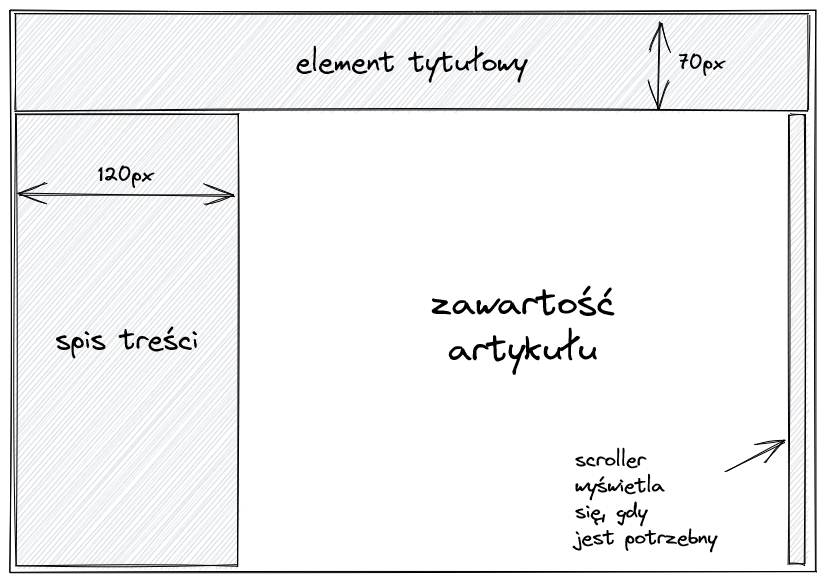
\includegraphics[width=0.7\textwidth]{zad2}
                \caption{Wymagany układ strony dla zadania~\ref{exc:layout}.}
                \label{fig:layout}
            \end{figure}

        \item\label{exc:native-input}
            (x pkt) Style native input.

        \item\label{exc:button-with-icon}
            (x pkt) Button with icon.

        \item\label{exc:range-with-knob}
        $\skull$ (x pkt) Slider component for Chrome, FF and Edge.

    \end{enumerate}
\end{document}

